\documentclass{article}
\usepackage{times}
\usepackage{lipsum}
\usepackage{graphicx}
\usepackage{mathtools}
\setlength{\parskip}{10pt plus 1pt minus 1pt}
\begin{document}
\begin{titlepage}
    \begin{center}
        \vspace*{1cm}
        \huge
        \textbf{Literature Review}
        
        \vspace{0.5cm}
        \LARGE
        Adversarial Examples in Machine Learning

        
        \vspace{1.5cm}
        
        \textbf{Rafael Carvalhaes Possas}
        
        \vfill
        
        \vspace{0.8cm}
        
        
        School of Information Technologies\\
        University of Sydney\\
        Australia\\

        
    \end{center}
\end{titlepage}
\section{Introduction}\label{sec:intro}

Artificial Intelligence efforts in the early days were focused in understanding the main principles behind human learning \cite{nielsen2016}. For instance, recognizing digits is a trivial and effortless job for most people, however, making a computer to be able to execute this same task might not be as easy as it is for an human being. Nevertheless, by discovering the pattern behind digit recognition, computers would also be able to start understanding broader classes of images/objects. This field of study nowadays is particularly known as "Computer Vision" \cite{goodfellow2016_book}.

The first studies for emulating the human brain started with the artificial neuron called \textit{perceptron} and these were developed in the 1950s and 1960s by the scientist Frank Roseblatt. Even though this model is not commonly used nowadays, it can be considered as one of the foundations for what is called \textit{Neural Networks} \cite{nielsen2016}. 

Neural Networks are a part of a broader set of machine learning algorithms. These are usually  focused in learning models that can represent certain beliefs, and through the use of what is called \textit{cost functions}, measure how well the model is actually representing the reality \cite{goodfellow2016_book}. Some of the most common machine learning tasks include: Classification, Regression and Clustering. The aforementioned problem of image recognition lies in the classification category, and, therefore, should be the type task studied in this work.

Recent advancements in computational power and developments of more advanced algorithms helped to popularize the use of computer vision in a wide variety of industries \cite{billovits}. This popularization raised some serious concerns regarding the robustness of these algorithms for executing such tasks. For instance, one would be able to attack a machine using a specific algorithm in order to make it behave for his/her own benefit.

It has been shown that several machine learning models, Neural Networks included, can miss-classify adversarial image examples \cite{goodfellow2014}. Such examples are usually created through applying small intentional perturbations to each pixel in a way that the classifier outputs the incorrect answer while, for human beings, the image is still recognizable as the same as before.

\section{Key Concepts}\label{sec:key_concepts}

\subsection{Neural Networks}\label{subsec:neural_deep}

In order to understand how neural networks can learn, lets firstly explain a single neuron through the \textit{perceptron} model. A perceptron works by transforming a set of inputs \{x\textsubscript{1},x\textsubscript{2},x\textsubscript{3}..\} into a specific output(s) through a function \textit{f(a)} that directly depends on the optimization of weights \{w\textsubscript{1},w\textsubscript{2},w\textsubscript{3}..\} and biases \{b\textsubscript{1},b\textsubscript{2},b\textsubscript{3}..\}\cite{nielsen2016}. Figure \ref{fig:perceptron}  helps to understand the intuition behind a single neuron.

The perceptron has a simple but yet powerful mathematical model. The weights can express the importance of a specific input for its neuron, moreover, a simple way of thinking about this is to understand that a perceptron is a device that makes decision by weighing up evidence \cite{nielsen2016}.
\begin{figure}[h!]
\centering
	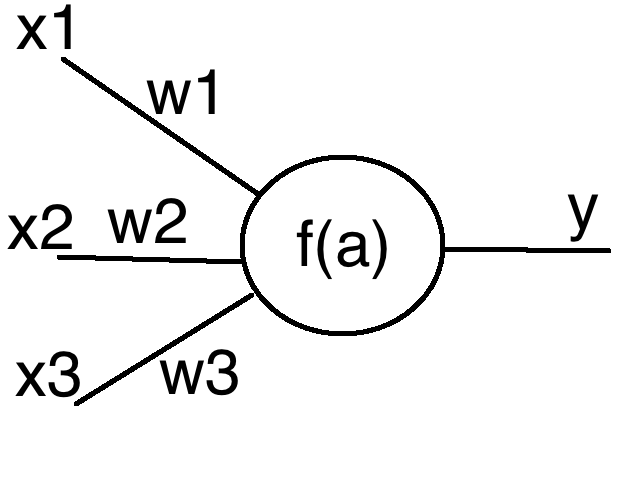
\includegraphics[scale=0.2]{perceptron.png}
\caption{A simple perceptron model}
\label{fig:perceptron}
\end{figure}

Even though the perceptron is a good model, it is far from complete. It has been illustrated already that different kinds of evidence can be used in order to teach the single neuron how to make decisions. Therefore, it would be feasible to put some neurons together in order to make the network capable of taking quite subtle decisions in regards to our input \cite{goodfellow2016_book}. These networks would be comprised by layers in which neuron activation would be responsible for identifying patterns and, thus, trigger different decisions with respect to different inputs \cite{nielsen2016}. 

However, non-linear models could also be represented by these layers. The aforementioned neuron model uses a simple linear model to represent its output. A more complex type called \textit{Sigmoid Neuron} could be used in order make the network capable of representing these so called non-linear models \cite{goodfellow2016_book}. The function used within this new neuron model would be the sigmoid function, which is known for its wide use in the logistic regression machine learning algorithm \cite{nielsen2016}. Besides, as it was already aforementioned, a cost function needs to be used within the training phase. For simple linear method, a quadratic cost function serves the purpose but for a logistic based neuron, most of the times the cost function that performs the best is the \textit{cross-entropy} cost \cite{nielsen2016}. The use of the cross-entropy cost function avoids the problem known as "leaning slowdown" commonly observed on neural networks with quadratic cost and sigmoid neuron \cite{nielsen2016}.

To sum up, it is crucial to understand how the outputs of the network varies with changes in any of its layers. A small change $\Delta$w will be applied to the network output when small changes occur on any of the weights. Next section will dive deep into how the use of an algorithm called \textit{backpropagation} leverages this rate of change to calculate and optimize the weights and biases of the model \cite{goodfellow2016_book}.
\begin{figure}[h!]
\centering
	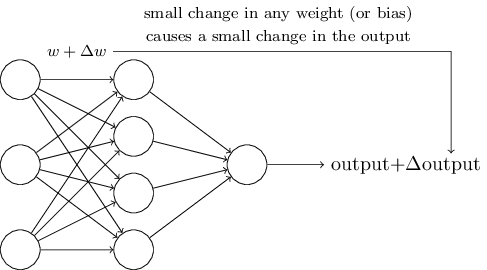
\includegraphics[scale=0.7]{net_change.png}
\caption{Output change with regards to layer(s) weight change \cite{nielsen2016}}
\label{fig:net_change}
\end{figure}

\subsection{Gradient Descent}\label{subsec:neural_deep}

Having the design of the network set, now it is needed to understand how a neural network can actually learn from its inputs. Suppose a training input \textit(x). The learning algorithm should be able to find weights and biases that best approximates the output \textit{y(x)} for all training inputs. Moreover, it should quantify during each iteration how close the output is from the actual result \cite{goodfellow2016_book}. Different machine learning algorithms require different cost functions \cite{nielsen2016}. This study will only focus on two methods for measuring training error: Quadradic and Coss-entropy cost functions.

The quadratic cost function is also know as mean squared error (MSE). This function is used on various machine learning algorithms and performs really well with linear problems \cite{nielsen2016}. The cost function should return small error when \textit{y(x}) is close to the real value and large value when it is far. The quadratic cost can be describe as the following equation:

$$C(\omega,b) \equiv \frac{1}{2n} \sum_{x} ||y(x) -a||^2 $$

The goal of training a neural network is to find weights and biases which minimize the selected cost function \textit{C(x)}. This goal can be achieved by using methods for Convex Optimization of functions \cite{goodfellow2014}. Gradient Descent is one of the methods for finding a global/local minimum of a function which minimizes its result. The algorithm consists of finding the rate of change of the cost function C(x) with regards to both weights $\omega$ and biases \textit{b}. This calculation yields what is a called a gradient vector which is subtracted from our current weight and biases in order to move the result towards the minimum. Lets imagine the gradient calculation as repeatedly computing $\nabla$C, and then moving in the opposite direction "falling down" the slope of the valley \cite{nielsen2016}.

\begin{figure}[h!]
\centering
	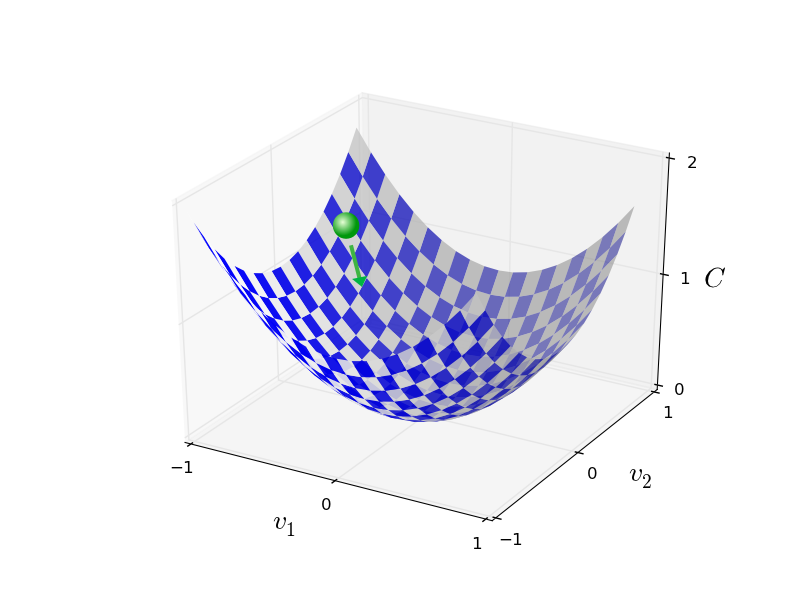
\includegraphics[scale=0.4]{valley_with_ball.png}
\caption{Gradient calculation representation \cite{nielsen2016}}
\label{fig:net_change}
\end{figure}

The main equations behind gradient descent are based on the partial derivatives of the cost function C(x). By taking the derivative with respect to the weights and biases, the algorithm is calculating the inclination of that point on a specific point of our cost function. On other words, this is can be seen as how fast the cost function is changing at that specific point \cite{nielsen2016}. Below are the equations used for the calculation of the gradient vector $\nabla$C.

$$\nabla C \equiv \frac{\partial C}{\partial \omega}, \frac{\partial C}{\partial b}$$
\subsection{Backpropagation}\label{subsec:backprop}
Backprop here
\subsection{Learning Slowdown and the Cross-Entropy Cost Function}\label{subsec:cross_entropy}
Even though the quadratic cost serves the purpose, it is a slow function for sigmoid neurons. The partial derivatives of the C(x) are given below.

$$\frac{\partial C}{\partial \omega} = (\alpha - y)\sigma'(z)x$$
$$\frac{\partial C}{\partial b} = (\alpha - y)\sigma'(z) $$

The result of the derivative with the respect to the weights depends on the derivative of the sigmoid function. This derivative yields a very low value when the neurons are near saturation, which causes a phenomenon known as "learning slowdown" \cite{nielsen2016}. Recall on shape of the sigmoid function on figure \ref{fig:sigmoid} that neuron activation is represent by both extremes of the function where the slope is almost flat and, therefore, the partial derivative will yield a very small value. Since the overall rate of change of our cost function is multiplied by this value, the network weights will have incremental small changes over each training iteration \cite{nielsen2016}.


\begin{figure}[h!]
\centering
	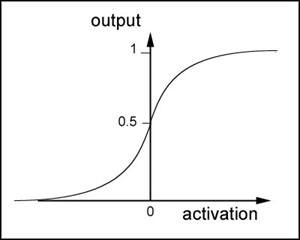
\includegraphics[scale=0.6]{sigmoid.jpg}
\caption{Sigmoid function Shape}
\label{fig:sigmoid}
\end{figure}
The solution for the learning slowdown lies in finding a cost function on which its derivative makes the $\sigma'(z)$ term disappear. In this case, the cost for a single example x would satisfy:

$$\frac{\partial C}{\partial \omega} = (\alpha - y)x$$
$$\frac{\partial C}{\partial b} = (\alpha - y) $$

Choosing a cost function that makes these equations true would capture the intuition that the greater the initial error, the faster the neuron learns eliminating completely the problem of a learning slowdown. Starting from these equations it is possible to derive the following equation known as the cross-entropy function \cite{nielsen2016}.

$$C = -\frac{1}{n} \sum_{x}[ yln(y) + (1-y)ln(1-y) ]$$

The intuitive meaning of cross-entropy comes from a field known as information theory. This function is a measure of expectation for a given output y(x). The cross-entropy will measure how "surprised" the algorithm will be on average when learning true value for \textit{y}. To sum up, the aforementioned derivations proves that the cross-entropy function is capable of dealing with the learning slowdown problem by eliminating the dependence on the cost function derivative from the term $\sigma'(z)$ and, thus, making the algorithm to learn at faster rates irrespective of where the current weights and biases are located \cite{goodfellow2016_book}.
\section{Neural Networks Properties}\label{sec: nn_props}

Deep Neural networks can be considered models with high expressiveness that can achieve extremely good performance on computer vision tasks. At the same time that being highly expressive helps them to succeed, it also drives them to learn solutions that are not easily understandable \cite{szegedy2013}. Usually there is a discontinuity in the input-output mappings of neural networks which can lead to miss-classification of images when the network prediction error is maximized \cite{gu2014}.The learning process of these networks through the backpropagation is rather complex and sometimes difficult to understand. Usually, the automatic discovered results through supervised learning are responsible for leading networks to acquire quite counter-intuitive properties \cite{szegedy2013}.

In order to understand the semantic meaning of individual units, researchers are currently focusing on understanding the factors leading to the activation of network neurons \cite{szegedy2013}. It has been argued that deep neural networks should be stable enough to provide robustness to small perturbation of its inputs. These should not be responsible for changing an image classification output. However, it has been found by mainly \cite{goodfellow2014} and \cite{szegedy2013} that minimal perturbations can indeed affect the network's predictions and, therefore, put down the assumption of local generalization over training inputs. Instead, global network level inspections methods should be more useful in the context of explaining classification decisions made by the model. This could be used, for instance, to identify the parts of the input that ended up leading to a correct classification of a given visual input \cite{szegedy2013}.

Generalization is usually achieved by making non-local assumptions of the training inputs \cite{gu2014}. A good model should be able to globally understand the patterns that leads to a specific class and, thus, use this knowledge on its future predictions. It is believed that deep stacks of non-linear layers are a way to have the model encoding a non-local generalization prior over the input space. Therefore, output units should be able to assign low probabilities to regions of the input space where no training examples are found within its vicinity \cite{szegedy2013}. The representation of low-probability "pockets" of space on images can lead to the creation of Adversarial examples. These are created by adding small localized perturbations on the input space which can ultimately lead to a miss-classification by the classifier. Due to this fact, it can be argued that deep neural networks are highly susceptible to local changes of the input space and, thus, are not able to have the expected generalization \cite{goodfellow2014}.

\section{Adversarial Examples}\label{sec: adversarial}

Adversarial Examples in machine learning have recently been studied by some researchers in the field. The question whether it is possible to fool these algorithms in a way that the output could favour one is still unanswered, however, there were some experiments that have shown that it is indeed possible to manipulate the results of these algorithms \cite{nguyen2015}. These experiments so far focused on creating models that would make adversarial examples to generalize and, thus, make deep neural networks (DNNs) to be highly susceptible to well-designed and small perturbations at the input layer \cite{gu2014}.

Deep Neural Networks have been able to achieve remarkable good accuracy in many classification problems \cite{krizhevsky2012}. Due to its extremely high number of non-linear units, these networks are able to automatically learn non-local generalization priors from data \cite{szegedy2013}. However, some methods for creating small perturbation have recently been discovered and, therefore, raises the question on whether these algorithms can be used in the real world without posing considerable threats to the community.

A careful literature review of the well known studies in this field have revealed three main techniques for creating adversarial examples and successfully attacking a machine learning algorithm. These will have a brief introduction below and a thorough analysis in the subsequent sections of this paper.

The first method for creating such examples is called "Fast Gradient Sign" and it was developed on \cite{goodfellow2014}. Generally speaking this method focuses on using gradient information to create small perturbations on inputs that can likely end up as a miss-classified example \cite{goodfellow2016}. In general, these are imperceptibly tiny perturbations that would not change the human understanding of the image class.

\subsection{Fast Gradient Sign}\label{subsec:fast_gradient}

Whether adversarial examples have non linear nature is still an open question \cite{dalvi2004}. However, \cite{goodfellow2014} showed that a simple linear model like the fast gradient sign can not only create adversarial examples but also explain why softmax regression is vulnerabe to these examples.  Most arbitrary points in space were miss-classified on the author experiments which shows that adversarial examples are not hard to find.

In order to understand the linear model behind the adversarial creation, it is needed to go back to the loss function explained on section \ref{sec:key_concepts}. The aim of the method is to change the loss function by a considerable value so the direction $\delta$ being moved is maximized.

$$ C(x + \delta)\approx C(x) + \delta . \nabla C$$

The intuition behind this formula can actually be easily explained. The goal is to create an $\alpha$ that emphasizes the pixels in the image with the highest importance, so the resulting perturbation of the image can likely lead to a miss-classified result. A way of making the product between $\delta$ and $\nabla$C big would be by making $\delta$ the \textit{sign} of the gradient. 

$$ C(x + \delta)\approx C(x) + sign(\nabla C)$$
\subsection{Rubbish Class}\label{subsec:rubbish}

Rubbish Class experiments suggested that deep models indeed behave too linearly since linear models become excessively confident when asked to extrapolate far from the training data.

\bibliographystyle{IEEEtran}
\bibliography{ref}



\end{document}